%% LyX 1.3 created this file.  For more info, see http://www.lyx.org/.
%% Do not edit unless you really know what you are doing.
\documentclass[english, 12pt]{article}
\usepackage{times}
%\usepackage{algorithm2e}
\usepackage{url}
\usepackage{bbm}
\usepackage[T1]{fontenc}
\usepackage[latin1]{inputenc}
\usepackage{geometry}
\geometry{verbose,letterpaper,tmargin=2cm,bmargin=2cm,lmargin=2cm,rmargin=2cm}
\usepackage{rotating}
\usepackage{color}
\usepackage{graphicx}
\usepackage{subcaption}
\usepackage{amsmath, amsthm, amssymb}
\usepackage{setspace}
\usepackage{lineno}
\usepackage{hyperref}
\usepackage{bbm}


%\usepackage{xr}
%\externaldocument{SCT-supp}

%\linenumbers
%\doublespacing
\onehalfspacing
%\usepackage[authoryear]{natbib}
\usepackage{natbib} \bibpunct{(}{)}{;}{author-year}{}{,}

%Pour les rajouts
\usepackage{color}
\definecolor{trustcolor}{rgb}{0,0,1}

\usepackage{dsfont}
\usepackage[warn]{textcomp}
\usepackage{adjustbox}
\usepackage{multirow}
\usepackage{graphicx}
\graphicspath{{figures/}}
\DeclareMathOperator*{\argmin}{\arg\!\min}

\let\tabbeg\tabular
\let\tabend\endtabular
\renewenvironment{tabular}{\begin{adjustbox}{max width=0.9\textwidth}\tabbeg}{\tabend\end{adjustbox}}

\makeatletter

%%%%%%%%%%%%%%%%%%%%%%%%%%%%%% LyX specific LaTeX commands.
%% Bold symbol macro for standard LaTeX users
%\newcommand{\boldsymbol}[1]{\mbox{\boldmath $#1$}}

%% Because html converters don't know tabularnewline
\providecommand{\tabularnewline}{\\}

\usepackage{babel}
\makeatother


\begin{document}


\title{Efficient toolkit implementing best practices for principal component analysis of population genetic data}
\author{Florian Priv\'e,$^{\text{1,}*}$ John J. McGrath,$^{\text{1,2,3}}$ and Bjarni J. Vilhj\'almsson$^{\text{1,}*}$}

\date{~ }
\maketitle

\noindent$^{\text{\sf 1}}$National Centre for Register-Based Research, Aarhus University, Aarhus, 8210, Denmark. \\
\noindent$^{\text{\sf 2}}$Queensland Brain Institute, University of Queensland, St. Lucia, 4072, Queensland, Australia. \\
\noindent$^{\text{\sf 3}}$Queensland Centre for Mental Health Research, The Park Centre for Mental Health, Wacol, 4076, Queensland, Australia.\\






\noindent$^\ast$To whom correspondence should be addressed.\\

\noindent Contacts:
\begin{itemize}
\item \url{florian.prive.21@gmail.com}
\item \url{john_mcgrath@qcmhr.uq.edu.au}
\item \url{bjv@econ.au.dk}
\end{itemize}

\newpage

\abstract{
Principal Component Analysis (PCA) of genetic data is routinely used to infer ancestry and control for population structure in various genetic analyses. However, conducting PCA in large populations is complicated, and there are several potential pitfalls. These pitfalls include (1) capturing Linkage Disequilibrium (LD) structure instead of population structure, (2) projected PCs that suffer from shrinkage bias when projecting PCA from a reference dataset to another independent dataset, and (3) detecting sample outliers. In this work, we explore these pitfalls of using PCA, and present efficient solutions to these pitfalls. Following applications to diverse datasets, we make recommendations for best practices and implement the proposed solutions in an efficient and user-friendly toolkit for performing these analyses in the R packages bigsnpr and bigutilsr.

For example, we show that PC18 to PC40 in the UK Biobank are capturing LD structure. Using our automatic algorithm for removing long-range LD region, we are able to recover only 17 PCs that capture population structure only. Therefore, we recommend using only 17 PCs from the UK Biobank. Another example: when projecting the PCA computed on the 1000 Genomes project, although PC1 to PC4 suffer from only moderate shrinkage (1.00-1.08), PC5 for example suffers from a shrinkage factor of 1.51 and PC10 from a shrinkage factor of 3.16. We provide a fast way to project new individuals that is mostly free of this shrinkage bias. We also show how to restrict to individuals that are genetically homogeneous based on PCA. 

Overall, we believe this work would be of interest for anyone using PCA in their analyses of genetic data.
}


%%%%%%%%%%%%%%%%%%%%%%%%%%%%%%%%%%%%%%%%%%%%%%%%%%%%%%%%%%%%%%%%%%%%%%%%%%%%%%%%

\newpage

\section{Introduction}

Principal Component Analysis (PCA) has been widely used in genetics has been used for many years and in many contexts such as e.g.\ to adjust for population structure in Genome-Wide Association Studies (GWAS) by adding PCs as covariates \cite[]{price2006principal} and to detect loci under selection based on PCA \cite[]{galinsky2016fast,luu2017pcadapt}.
Much work has been devoted to developing scalable algorithms to compute PCA on data as large as the UK Biobank \cite[]{bycroft2017genome}, which is now possible thanks to software such as FastPCA (fast mode), FlashPCA2, PLINK 2.0 (approx mode), bigstatsr/bigsnpr and TeraPCA \cite[]{galinsky2016fast,abraham2017flashpca2,chang2015second,prive2017efficient,bose2019terapca}.

However, some pitfalls related to PCA of genotype data has been documented and we recall them here. This includes some possible lack of precision of computed PCs of software such as FastPCA and PLINK 2.0, which is not an issue for FlashPCA2 and bigstatsr/bigsnpr \cite[]{abraham2017flashpca2,prive2017efficient}.
This also includes capturing Linkage Disequilibrium (LD) structure in PCA instead of population structure only \cite[]{price2008long,abdellaoui2013population,prive2017efficient}. This leads to e.g.\ an over-correction of GWAS variants within long-range LD regions [REWORD/PRECISE].
Finally, another issue may arise when projecting PCs of a reference dataset to another study dataset: projected PCs are shrunk towards 0 in the new dataset \cite[]{lee2010convergence,wang2015improved,zhang2019fast}. This shrinkage makes it dangerous to use the projected PCs for analysis such as PC regression, ancestry detection and GWAS [REWORD/PRECISE].

In this paper, we derive a new implementation of PCA that can be used directly on bed/bim/fam PLINK files with some missing values, which is available in R package bigsnpr v1.0.0. Then, we recall some of the pitfalls of PCA computation on genotype data and provide efficient solutions to these issues, such as accouting for LD structure in PCA, detecting outliers [NOT INTRODUCED BEFORE] and projecting PCs to another study sample without shrinkage bias.



%%%%%%%%%%%%%%%%%%%%%%%%%%%%%%%%%%%%%%%%%%%%%%%%%%%%%%%%%%%%%%%%%%%%%%%%%%%%%%%%

\section{Material and Methods}

\subsection{PCA with missing values}

When there is no missing value, we compute the partial Singular Value Decomposition (SVD) $U \Delta V^T$ of the scaled genotype matrix $\tilde{G}_{i,j} = \frac{G_{i,j} - 2 \hat{f_j}}{\sqrt{2 \hat{f_j} (1 - \hat{f_j})}}$ where $G_{i,j}$ is the allele count (genotype) of individual $i$ and variant $j$, and $\hat{f_j}$ is the estimated allele frequency of variant $j$ ($2 \hat{f_j}$ is the mean allele count of variant $j$). Then, $U \Delta$ are the first $K$ PC scores and $V$ are the first $K$ PC loadings, where $K$ is the number of PCs computed (e.g.\ $K=20$).

When there is some missing values, we compute the partial SVD similarly, except that missing values are replaced by the variant means (i.e.\ $G_{i,j} - 2 \hat{f_j} = 0$ when $G_{i,j}$ is missing) and  the $\hat{f_j}$ for each variant are estimated using only non missing values of each variant.
Note that this decomposition is equivalent to the decomposition presented above after imputation by the variant means [SURE?].

\subsection{Robust Mahalanobis distance \label{maha}}

In this paper, for many applications, we use the pairwise orthogonalized Gnanadesikan-Kettenrin robust Mahalanobis distance as implemented in function \texttt{covRob} of R package robust with parameter \texttt{estim = "pairwiseGK"} \cite[]{gnanadesikan1972robust,yohai1988high,maronna2002robust,todorov2009object}. We reexport this function in R package bigutilsr for convenience.

\subsection{Detecting LD structure in PCA}

For detecting outlier variants in PCA that are due to long-range Linkage Disequilibrium (LD) regions, we use a slightly modified version of the procedure described by \cite{prive2017efficient}. 
To summarise the contribution of each variant in all PC loadings, we compute the robust Mahalanobis distances (Section \ref{maha}) of PC loadings.  
This captures both population-differentiating variants as well as long-range LD regions. 
Then, to capture consecutive outliers that corresponds to long-range LD regions, we apply a Gaussian smoothing to these statistics.

Finally, to choose the threshold of outlierness based on the previously described statistics, we use a modified version of Tukey's rule, a standard rule for detecting outliers \cite[]{tukey77}. 
The standard upper limit defined by Tukey's rule is $q_{75\%}(x) + 1.5 \cdot IQR(x)$, where $x$ is the vector of computed statistics and $IQR(x) = q_{75\%}(x) - q_{25\%}(x)$ is the interquartile range.
However, there are two pitfalls when using Tukey's rule. First, Tukey's rule assumes a normally distributed sample. For example, when the data is skewed, it does not work that well. We account for skewness using the medcouple \cite[]{hubert2008adjusted}. Standard Tukey's rule also uses a fixed coefficient (1.5) that does not account for multiple testing, which means that for large samples, there are always some outliers detected when using 1.5. 
To solve these two issues, we implement \texttt{tukey\_mc\_up} in R package bigutilsr and use it here, which accounts both for skewness and multiple testing by default.

\subsection{Detecting outlier samples in PCA}

We propose [BOF] different outlier detection techniques for PCA.


For detecting outlier samples in PCA, we use the Local Outlier Factor (LOF) on PCs \cite[]{breunig2000lof}. To make it robust to the choice of the number of nearest neighbours (kNN), we take the maximum value of the statistic computed with kNN $\in$ \{4, 5, 6, 7, 8\}. We do not use larger values for `kNN' because it would remove small ancestry groups (e.g.\ composed of 10-15 people only). We make use of the fast K nearest neighbours implementation of R package nabor to implement the LOF statistic efficiently in our new R package bigutilsr \cite[]{elseberg2012comparison}.
 
For detecting samples that have a different ancestry from most of the samples in the data, we compute the pairwise orthogonalized Gnanadesikan-Kettenrin robust Mahalanobis distance of PCs \cite[]{gnanadesikan1972robust,maronna2002robust}, and do not include individuals whose log-distance is larger than some threshold determined based on visual inspection [DO IT AUTOMATIC?].



\subsection{Subsetted version of 1000G data [RENAME?]\label{1000G}}

We provide a subsetted version of the 1000 genomes (1000G) project data \cite[]{10002015global,meyer2019genotype}.
Variants are restricted to the ones in common with HapMap3 and UK Biobank \cite[]{international2010integrating,bycroft2017genome}. 
Moreover, we apply some quality control filters; we remove variants having a minor allele frequency < 0.01, variants or individuals with more than 10\% missing value, variants with P-value of the Hardy-Weinberg exact test < $10^{-50}$, and non-autosomal variants. 
To remove related individuals with second-degree relationship or more, we apply KING cutoff of 0.0884 to the data using PLINK 2.0 \cite[]{manichaikul2010robust,chang2015second}.
This results in 2490 individuals of the 1000G project (phase 3) in PLINK bed/bim/fam format. 
Resulting PLINK files and R code to generate these files are available at \url{https://doi.org/10.6084/m9.figshare.9208979.v3}. 
To easily download these data, we provide a function called \texttt{download\_1000G} in R package bigsnpr.


\subsection{Projecting PCs from a reference dataset \label{proj}}

%[SEPARATE STEPS?]

To project PCs of a reference dataset (e.g.\ 1000G) to a target genotype dataset, we implement the following 3 steps in function \texttt{bed\_projectPCA} of package bigsnpr: 1) matching the variants of each dataset, including removing ambiguous alleles [A/T] and [C/G], and matching strand and direction of the alleles; 2) computing PCA of the reference dataset using the matched variants only; 3) projecting computed PCs to the target data using an optimised implementation (see Supplementary Materials) of the Online Augmentation, Decomposition, and Procrustes (OADP) transformation \cite[]{zhang2019fast}.

\subsection{Ancestry matching \label{ancestry}}

We use the 1000 Genomes (1000G) Project data (section \ref{1000G}) to infer the ancestry of individuals from a study dataset following the following steps: 1) we compute the robust center and covariance parameters of the Mahalanobis distance (section \ref{maha}) for each of the 26 populations of the 10000G data; 2) we project individuals from the study dataset onto the PCA space computed using the 1000G data (section \ref{proj}); 3) we compute the Mahalanobis distance for each projected individual of the study data and each population of the 1000G data (using the center and covariance parameters computed previously); 4) we derive p-values from those distances, as they are approximately chi-squared distributed with the number of PCs used for computing the distances as degrees of freedom; 5) we affect each individual to the largest corresponding p-value (smallest distance), but discard individuals whose maximum p-value is less than 0.05 (i.e.\ individuals far from every population of the 1000G data). 

%%%%%%%%%%%%%%%%%%%%%%%%%%%%%%%%%%%%%%%%%%%%%%%%%%%%%%%%%%%%%%%%%%%%%%%%%%%%%%%%

\section{Results}

\subsection{Projecting PCs from a reference dataset}

We use 60\% of individuals in the 1000G data (section \ref{1000G}) to compute the PCA ($K=20$ PCs). Then, we project the remaining 40\% individuals using three methods: 1/ simply multiplying the genotypes of these individuals by the previously computed loadings, 2/ correcting the simple projections using asymptotic shrinkage factors as determined by R package hdpca v1.0.0 \cite[]{dey2019asymptotic} and 3/ the OADP projection (section \ref{proj}). 
When simply projecting using loadings, there is no apparent shrinkage for PC1 and PC2, a weak [REWORD?] shrinkage for PC3 and PC4, and a large shrinkage for PC5 to PC8 (Figure \ref{fig:proj1000G}).
In contrast, there is no apparent shrinkage when projecting new individuals with OADP (Figure \ref{fig:proj1000G}).
Simple projection is affected even more by this shrinkage for PC9 to PC20, while OADP appears free of this issue (Figure \ref{fig:proj1000G-2}).
We show the same results when projecting the full UK Biobank data onto PCA computed using 1000G data  (Figure \ref{fig:proj1000G-5}).
When correcting projected PC scores with asymptotic shrinkage factors, bias is smaller than when simply projecting loadings, yet, it is apparent for PC7-8 and PC11-12 (Figure \ref{fig:proj1000G-3}).
Finally, to assess if OADP could be used to project individuals that are related to some individuals that were used to compute PCA, we projected these individuals (as if we were projecting their monozygotic twins) using OADP. Projections of related individuals using OADP shows some reverse [REWORD?] shrinkage (Figure \ref{fig:proj1000G-4}).

\begin{figure}[!htpb]
\centerline{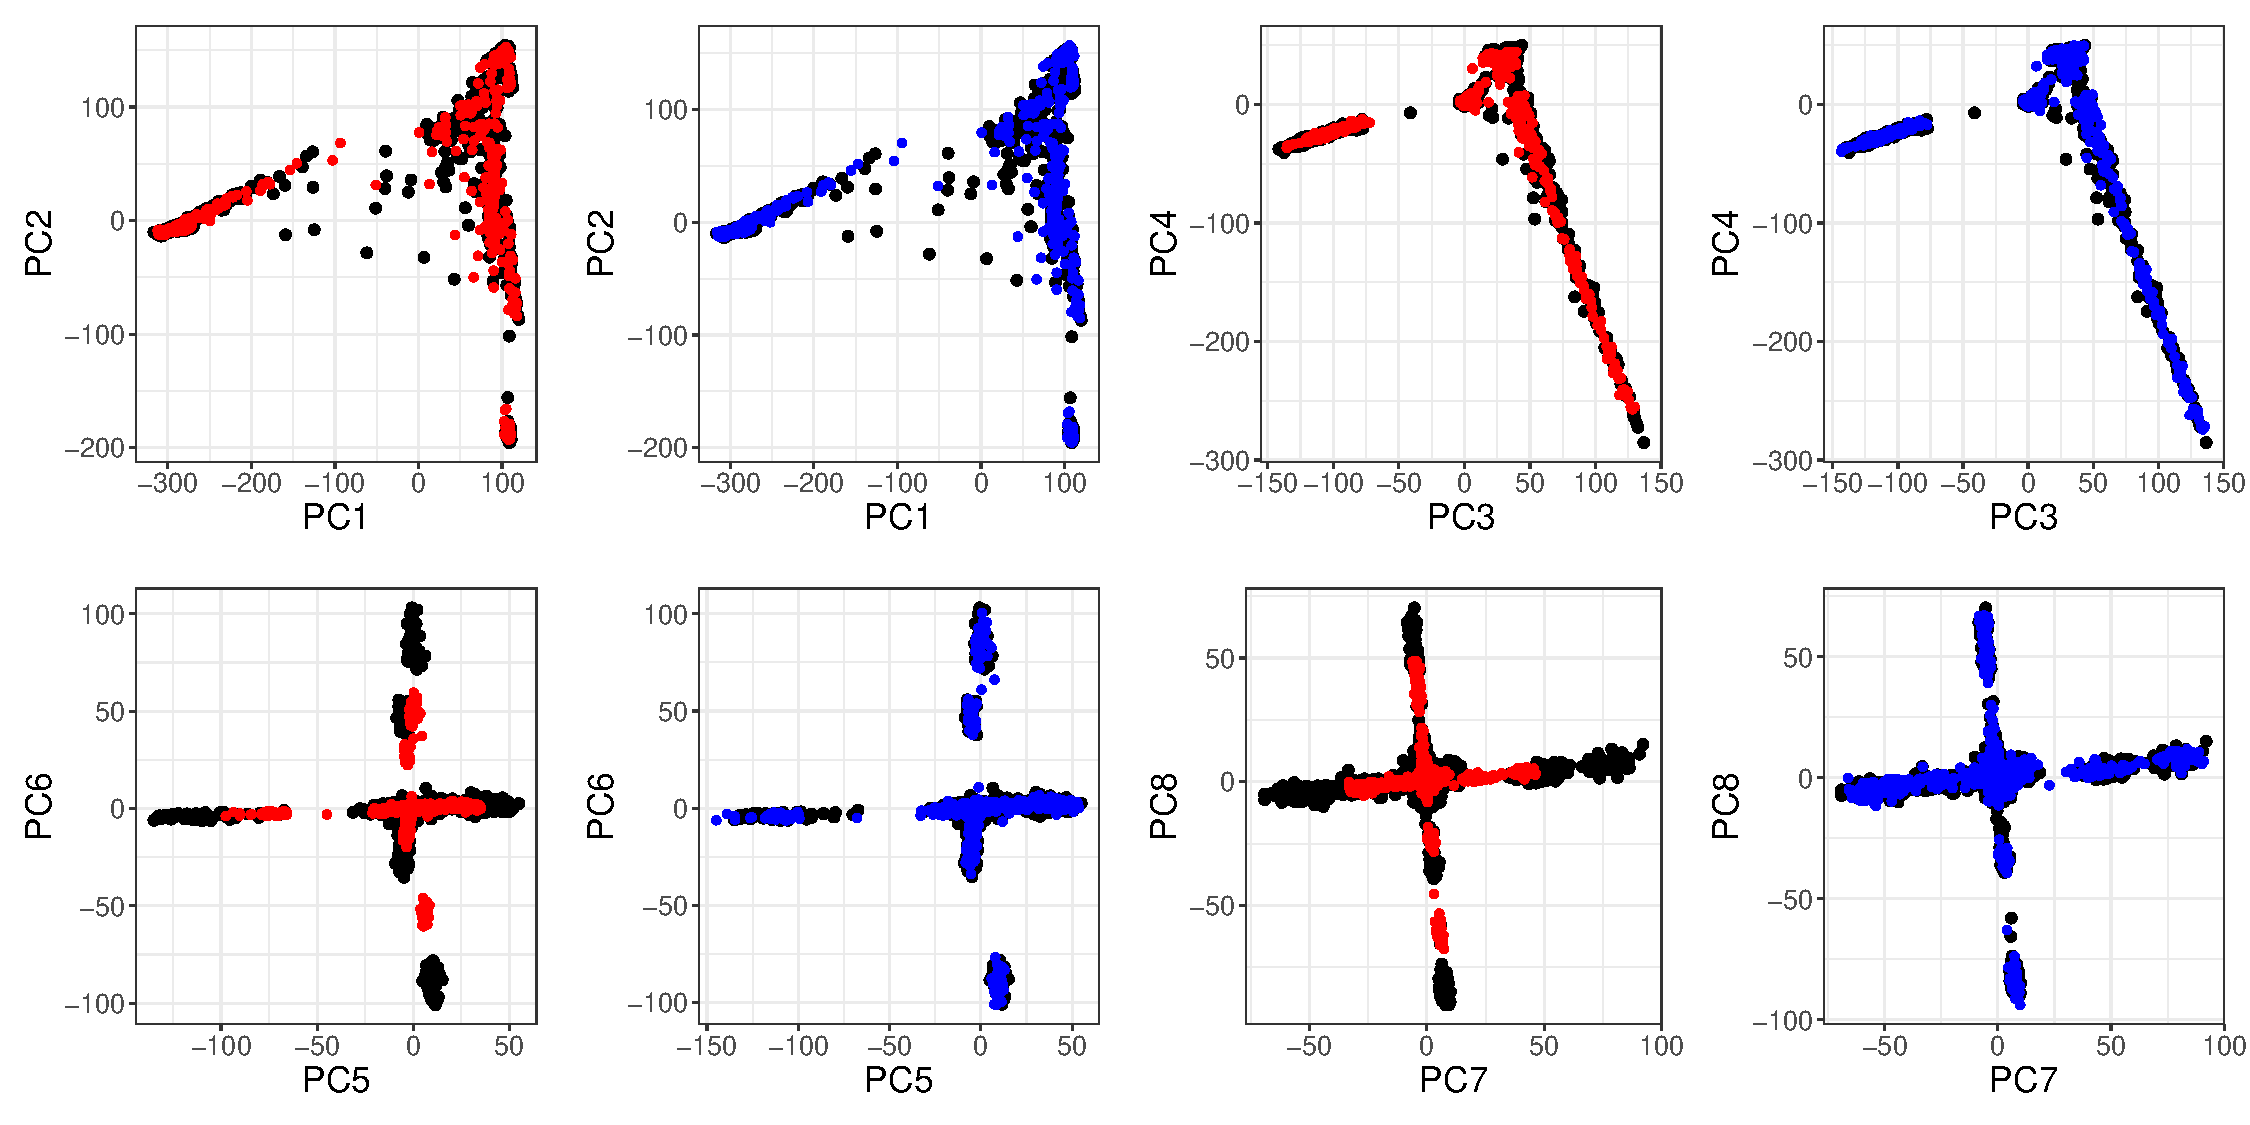
\includegraphics[width=0.8\textwidth]{proj1000G-PC1-8.pdf}}
\caption{Principal Component (PC) scores 1 to 8 of the 1000 Genomes project.
Black points are the 60\% individuals used for computing PCA.
Red points are the 40\% remaining individuals, projected by simply multiplying their genotypes by the corresponding PC loadings.
Blue points are the 40\% remaining individuals, projected using the Online Augmentation, Decomposition, and Procrustes (OADP) transformation.
\label{fig:proj1000G}}
\end{figure}

\subsection{Ancestry matching}

[REDO WITH OUTLIER REMOVAL?]

We performed ancestry estimation of the individuals in the UK Biobank using the 1000G data (Section \ref{ancestry}), discarding individuals with unknown ancestry or mixed ancestry. 
We did not infer ancestry for 15.5\% of UK Biobank that had a maximum p-value smaller than 0.05 (Figure \ref{fig:ancestry-pval}). 
More precisely, among ``White'', ``British'' and ``Irish'' ancestries, this represented respectively 20.4\%, 10.5\% and 19.8\%, while this represented between 48.5\% (``Chinese'') and 81.4\% (``Bangladeshi'') for other populations. 
In other words, most of the UK Biobank individual who self-reports as ``Bangladeshi'' could not be attributed to any 1000G population, although 1000G data includes several ``Bengali in Bangladesh'' (SAS\_BEB).
Only 10 people out of 401,048 were wrongly classified in ``super'' population of the 1000G; e.g.\ one Chinese person was classified as European by our method (Table \ref{tab:ancestry-pred}). 
Moreover, our method is able to accurately differentiate between sub-continental populations such as differentiating between Pakistani, Bangladeshi and Chinese people (Table \ref{tab:ancestry-pred}).

% latex table generated in R 3.6.0 by xtable 1.8-4 package
% Sat Oct 19 22:53:58 2019
\begin{table}[ht]
\centering
\caption{Self-reported ancestry (top) of UKBB individuals and their matching to 1000G populations (left) by our method. See the description of 1000G populations at \url{https://www.internationalgenome.org/category/population/}.} 
\label{tab:ancestry-pred}
\begin{tabular}{|l|c|c|c|c|c|c|c|c|c|c|c|c|c|}
  \hline
 & British & Irish & White & Other White & Indian & Pakistani & Bangladeshi & Chinese & Other Asian & Caribbean & African & Other Black & NA \\ 
  \hline
AFR\_ACB &  &  &  &  &  &  &  &  &  & 1687 & 580 & 28 & 252 \\ 
  AFR\_ASW &  &  &  &  &  &  &  &  &  & 365 & 12 & 12 & 41 \\ 
  AFR\_ESN &  &  &  &  &  &  &  &  &  &  & 103 &  & 16 \\ 
  AFR\_GWD &  &  &  &  &  &  &  &  &  &  & 12 &  & 5 \\ 
  AFR\_LWK &  &  &  &  &  &  &  &  &  &  & 33 &  & 6 \\ 
  AFR\_MSL &  &  &  &  &  &  &  &  &  &  & 23 &  & 2 \\ 
  AFR\_YRI &  &  &  &  &  &  &  &  &  & 4 & 403 & 3 & 66 \\ 
   \hline
AMR\_CLM & 1 &  &  & 47 &  &  &  &  &  &  &  &  & 127 \\ 
  AMR\_MXL &  &  & 1 & 3 &  &  &  &  &  &  &  &  & 21 \\ 
  AMR\_PEL &  &  &  & 1 &  &  &  &  &  &  &  &  & 14 \\ 
   \hline
EAS\_CDX &  &  &  &  &  &  &  & 1 &  &  &  &  &  \\ 
  EAS\_CHB & 1 &  &  &  &  &  &  & 369 & 10 &  &  &  & 9 \\ 
  EAS\_CHS &  &  &  &  &  &  &  & 398 & 8 &  &  &  & 18 \\ 
  EAS\_JPT &  &  &  &  &  &  &  & 2 & 23 &  &  &  & 114 \\ 
  EAS\_KHV &  &  &  &  &  &  &  & 3 & 14 &  &  &  & 19 \\ 
   \hline
EUR\_CEU & 323808 & 6547 & 348 & 4904 &  &  &  & 1 &  &  &  &  & 1358 \\ 
  EUR\_FIN & 3 &  &  & 115 &  &  &  &  &  &  &  &  & 1 \\ 
  EUR\_GBR & 62059 & 3682 & 79 & 482 &  &  &  &  &  &  & 1 &  & 268 \\ 
  EUR\_IBS & 35 &  & 5 & 494 &  &  &  &  &  &  &  &  & 10 \\ 
  EUR\_TSI & 20 &  & 1 & 156 &  &  &  &  &  &  &  &  & 3 \\ 
   \hline
SAS\_BEB &  &  &  &  & 10 &  & 41 &  &  &  &  &  & 4 \\ 
  SAS\_GIH &  &  &  &  & 292 &  &  &  &  &  &  &  & 3 \\ 
  SAS\_ITU & 1 &  &  &  & 270 & 1 &  &  & 224 & 2 &  &  & 69 \\ 
  SAS\_PJL &  &  &  &  & 1406 & 641 &  &  & 82 & 2 &  &  & 147 \\ 
  SAS\_STU &  &  &  &  & 39 &  &  &  & 198 &  &  &  & 47 \\ 
   \hline
NA & 45101 & 2526 & 111 & 9614 & 3699 & 1106 & 180 & 730 & 1188 & 2237 & 2037 & 75 & 7051 \\ 
   \hline
  \end{tabular}
\end{table}

\noindent[OKAY TO CLASSIFY SOME OTHER WHITE AS CENTRAL/SOUTH AMERICANS?]
 
\noindent[INCLUDE RESULTS FOR SIMPLE PROJ? -> HIST PVAL BAD -> 38\% NOT MATCHED, ESP PAKISTANI] 

We also projected individuals using the OADP projection and then applied our ancestry detection technique to other datasets. 
When applied to the European individuals of the POPRES data \cite[]{nelson2008population}, we show that 56.5\% of individuals could not be matched to one of the 26 populations of the 1000G data (Table \ref{tab:ancestry-pred-popres}). 
This is particularly dramatic for all East-Europeans, whose only 11 people could be matched out of 179 (6.1\%).
Moreover, even though 1000G data include several ``Toscani in Italia'' (EUR\_TSI), we were able to match 14.2\% of Italians only.
Nevertheless, for individuals that we could match, they were all identified as European ancestry. We could also identify accurately sub-regions of Europe; e.g.\ all Spanish and Portugese individuals that we could match (73.1\%) were identified as ``Iberian Population in Spain'' (EUR\_IBS, Table \ref{tab:ancestry-pred-popres}).
Finally, we also projected and matched people from a case-control cohort for celiac disease composed of four European countries: Italy, the Netherlands, the UK and Finland \cite[]{dubois2010multiple}. 
Among UK individuals, 5397 (79.9\%) were matched to either ``Utah Residents with Northern and Western European Ancestry'' (EUR\_CEU) or ``British in England and Scotland'' (EUR\_GBR), 10 (0.2\%) to other European populations, 1 to ``Mexican Ancestry from Los Angeles USA'' (AMR\_MXL) and 1346 (19.9\%) could not be matched (Table \ref{tab:ancestry-pred-celiac}).
Among Finns, 1543 (62.4\%) were matched to ``Finnish in Finland'' (EUR\_FIN), 6 (0.3\%) to other European populations, and 922 (37.3\%) could not be matched.
Among Italians, 229 (22\%) were matched to EUR\_TSI, 15 (1.5\%) to EUR\_IBS and 795 (76.5\%) could not be matched (Table \ref{tab:ancestry-pred-celiac}).

%%%%%%%%%%%%%%%%%%%%%%%%%%%%%%%%%%%%%%%%%%%%%%%%%%%%%%%%%%%%%%%%%%%%%%%%%%%%%%%%

\section{Discussion}

\noindent[LIMITATION: RUN MULTIPLE TIMES / FAIL TO SPEED UP]

\noindent[LIMITATION 2: FAIL TO PROJECT RELATED INDIVIDUALS WITH OADP.]

\noindent[LIMITATION 3: FAIL TO AUTOMATICALLY DETECT OUTLIER SAMPLES.]

\noindent[DISCUSS ABOUT $K''=K'=K$? FASTER, EASIER, DO NOT WANT MORE DIM?]



\subsection{Conclusion}




%%%%%%%%%%%%%%%%%%%%%%%%%%%%%%%%%%%%%%%%%%%%%%%%%%%%%%%%%%%%%%%%%%%%%%%%%%%%%%%%

%\newpage

\section*{Funding}

\section*{Acknowledgements}

This research has been conducted using the UK Biobank Resource under Application Number 25589.

~\\ \textit{Conflict of Interest:} none declared.

%%%%%%%%%%%%%%%%%%%%%%%%%%%%%%%%%%%%%%%%%%%%%%%%%%%%%%%%%%%%%%%%%%%%%%%%%%%%%%%%

%\newpage

\bibliographystyle{natbib}
\bibliography{refs}

%%%%%%%%%%%%%%%%%%%%%%%%%%%%%%%%%%%%%%%%%%%%%%%%%%%%%%%%%%%%%%%%%%%%%%%%%%%%%%%%

\newpage
\section*{Supplementary Materials}

\renewcommand{\thefigure}{S\arabic{figure}}
\setcounter{figure}{0}
\renewcommand{\thetable}{S\arabic{table}}
\setcounter{table}{0}

\subsection*{Optimised OADP transformation}

We implement an optimised version of the Online Augmentation, Decomposition, and Procrustes (OADP) transformation when using $K''=K'=K$ \cite[]{zhang2019fast}.
We assume that the $K$-partial Singular Value Decomposition (SVD) of the reference matrix $X$ (of size $n \times p$) has been computed as $U \Delta V^T$. There are several steps to perform OADP transformation for each sample $y$ (of size $1 \times p$) of target matrix $Y$ (of size $m \times p$):
\begin{enumerate}
\item Calculate $l = y \cdot V$ (of size $1 \times K$), where $V$ are the K PC loadings. And $g = y \cdot h^T$ (of size $1 \times 1$), where $h = (y - l \cdot V^T) / ||y - l \cdot V^T||_2$. Actually, $||y - l \cdot V^T||_2^2 = y \cdot y^T - 2 \cdot y \cdot V \cdot l^T  + l \cdot V^T \cdot V \cdot l^T = y \cdot y^T - l \cdot l^T$ and $y \cdot (y - l \cdot V^T)^T = y \cdot y^T - y \cdot V \cdot l^T = y \cdot y^T - l \cdot l^T$. Then $g = \sqrt{y \cdot y^T - l \cdot l^T}$.
\item Calculate $Q^T Q$ where $$Q = \begin{bmatrix} \Delta & l^T \\ 0 & g \end{bmatrix}$$ so that $$Q^TQ = \begin{bmatrix} \Delta^2 & \Delta \cdot l^T \\ l \cdot \Delta & g^2 + l \cdot l^T \end{bmatrix} = \begin{bmatrix} \Delta^2 & \Delta \cdot l^T \\ l \cdot \Delta & y \cdot y^T \end{bmatrix}.$$ Note that we do not actually need to compute $g$, and that we can update the last row and column of $Q^T Q$ instead of computing it from an updated version of $Q$.
\item Get the eigen decomposition $Q^T Q = V' {\Delta'}^2 {V'}^T$ (truncated to $K$ components out of the $K+1$). Let us denote $V_2 = V' {\Delta'}$.
\item Calculate $$\begin{bmatrix} \widetilde{U} \\ \widetilde{u}  \end{bmatrix} = \begin{bmatrix} U & 0 \\ 0 & 1 \end{bmatrix} V_2 = \begin{bmatrix} U V_2[1{:}K,~] \\ V_2[K{+}1,~] \end{bmatrix} $$
\item Find the Procrustes transformation from $\widetilde{U}$ to $U \Delta$. As $\widetilde{U}$ and $U \Delta$ have both their columns centered already (since $U$ does), the Procrustes transformation $\rho \widetilde{U} A$, where $\rho$ is a scaling coefficient and $A$ is an orthonomal projection matrix that minimise the Frobenius norm of $(\rho \widetilde{U} A - U)$, is given by $A = V'' {U''}^T$ and $\rho = \frac{\text{trace}(\Delta'')}{\text{trace}(\widetilde{U}^T \widetilde{U})}$ where $U'' \Delta'' {V''}^T$ is the full SVD of $(U \Delta)^T \widetilde{U}$ \cite[]{wang2015improved}. 
As $U^T U = I$, we note that $(U \Delta)^T \widetilde{U} = \Delta V_2[1{:}K,~]$ and that $\rho = \frac{\text{trace}(\Delta'')}{\text{trace}({V_2[1{:}K,~]}^T V_2[1{:}K,~])}$, therefore we do not need to explicitly compute $\widetilde{U}$. 
\item Apply the previous transformation to $\widetilde{u}$ to get the projection of $y$ in the reference PCA space (i.e.\ $\rho \widetilde{u} A$).
\end{enumerate}


%%%%%%%%%%%%%%%%%%%%%%%%%%%%%%%%%%%%%%%%%%%%%%%%%%%%%%%%%%%%%%%%%%%%%%%%%%%%%%%%

\clearpage

\subsection*{Supplementary figures}

\vspace*{1em}

\begin{figure}[!htpb]
\centerline{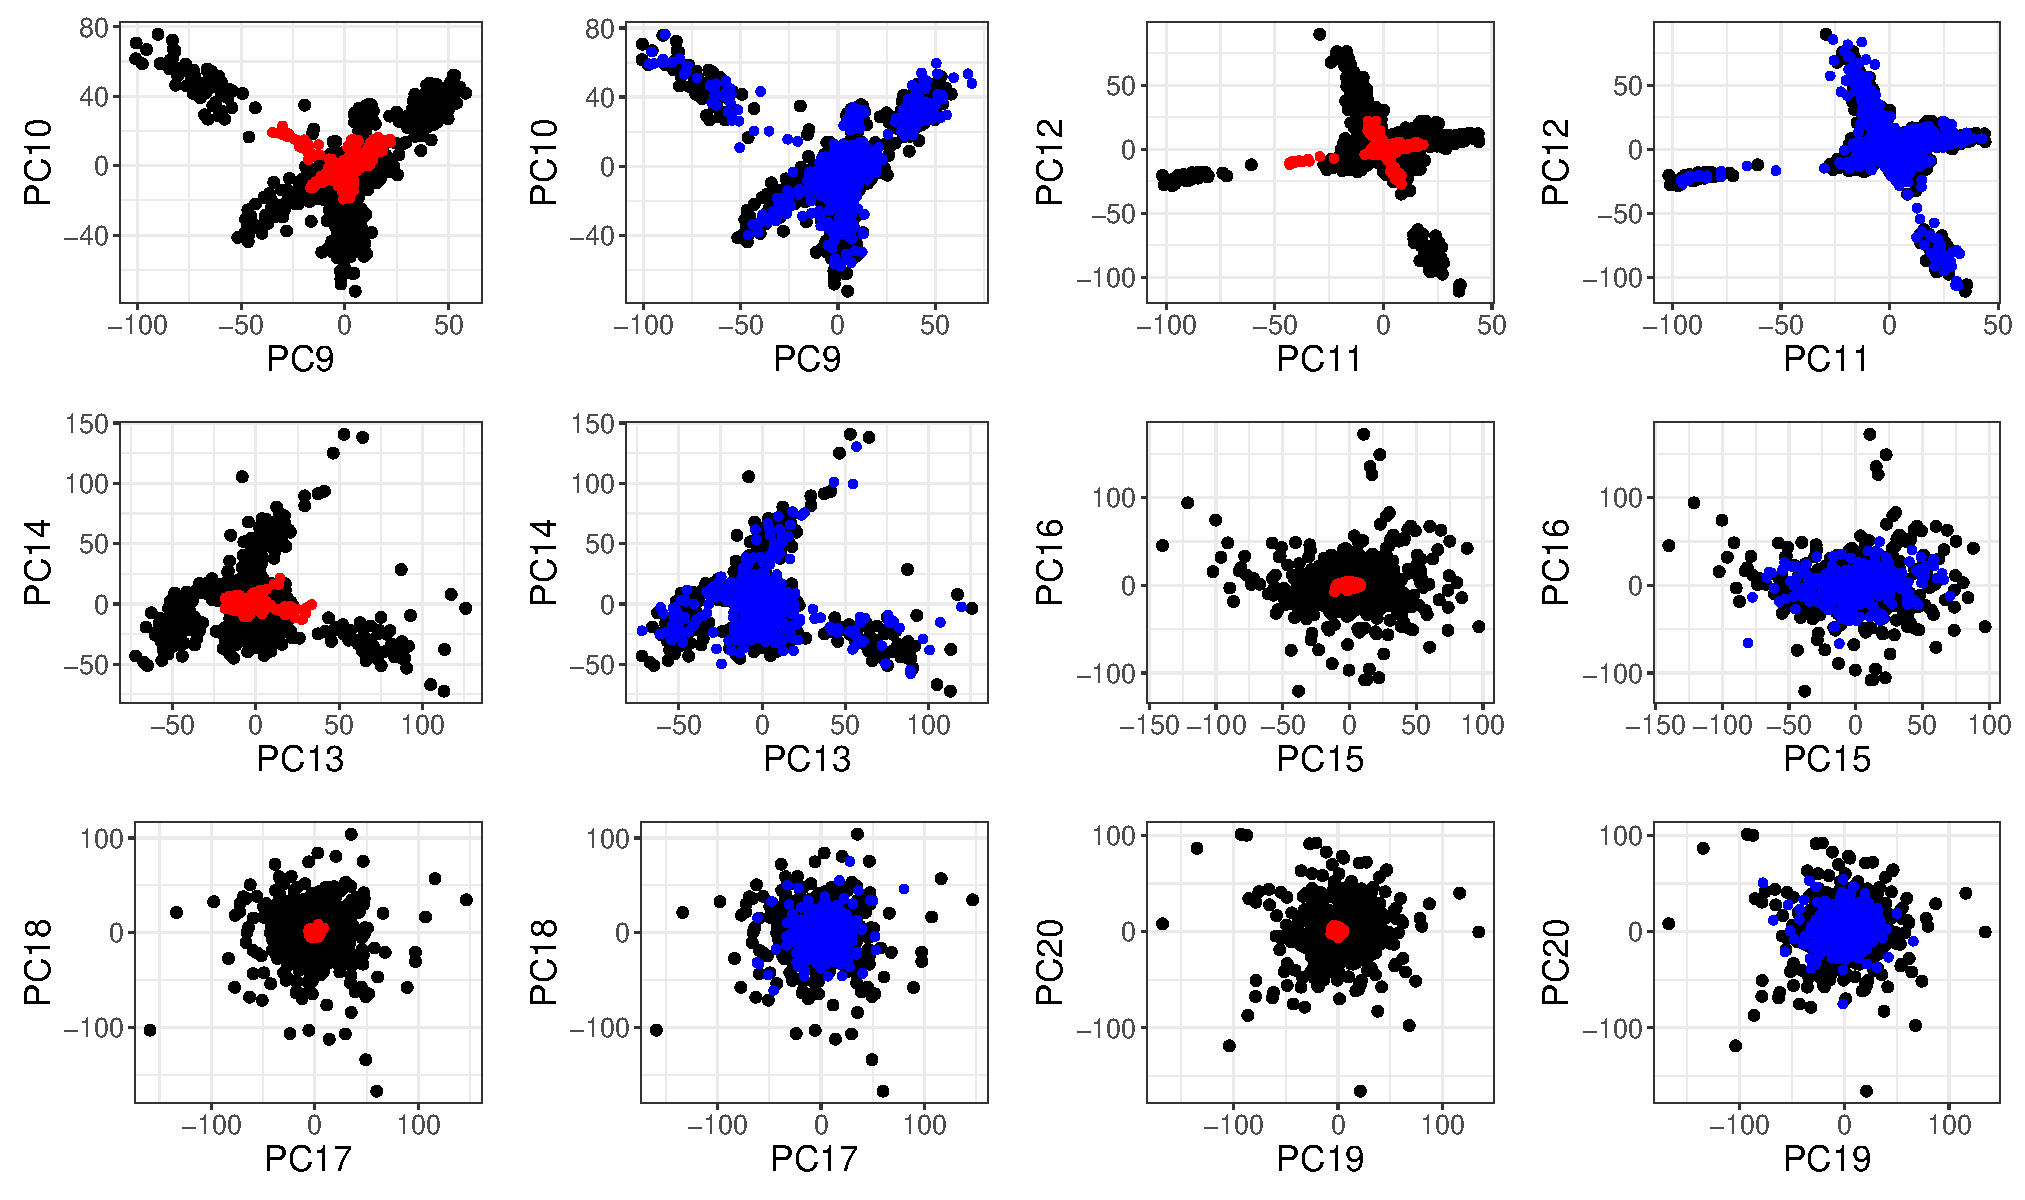
\includegraphics[width=0.9\textwidth]{proj1000G-PC9-20.pdf}}
\caption{Principal Component (PC) scores 9 to 20 of the 1000 Genomes project.
Black points are the 60\% individuals used for computing PCA.
Red points are the 40\% remaining individuals, projected by simply multiplying their genotypes by the corresponding PC loadings.
Blue points are the 40\% remaining individuals, projected using the Online Augmentation, Decomposition, and Procrustes (OADP) transformation.
\label{fig:proj1000G-2}}
\end{figure}

\vspace*{1em}

\begin{figure}[!htpb]
\centerline{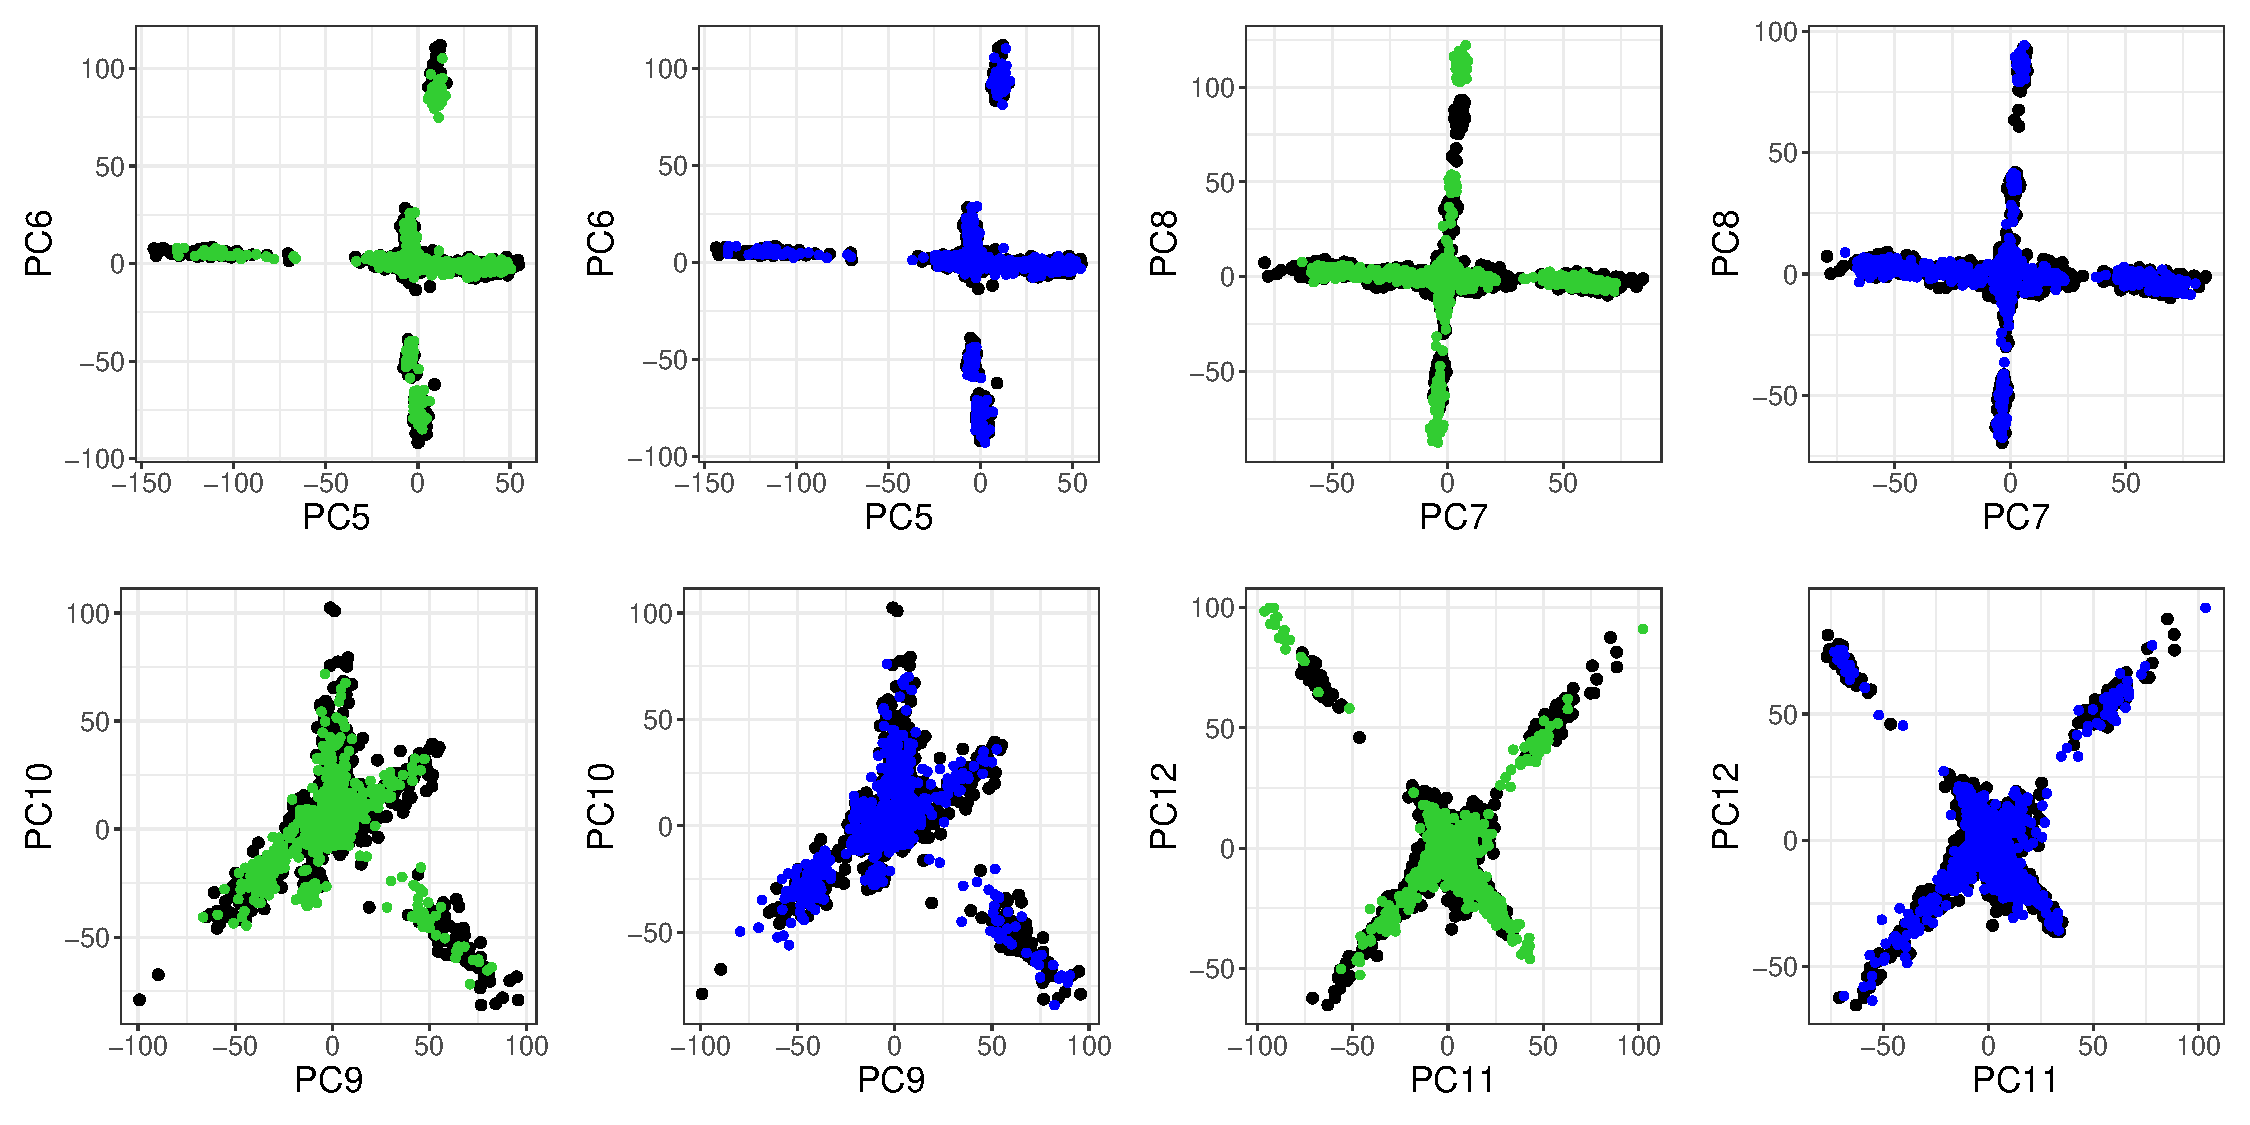
\includegraphics[width=0.9\textwidth]{proj1000G-PC5-12.pdf}}
\caption{Principal Component (PC) scores 5 to 12 of the 1000 Genomes project.
Black points are the 60\% individuals used for computing PCA.
Green points are the 40\% remaining individuals, projected by multiplying their genotypes by the corresponding PC loadings, further corrected using theoritical asymptotic shrinkage factors.
Blue points are the 40\% remaining individuals, projected using the Online Augmentation, Decomposition, and Procrustes (OADP) transformation.
\label{fig:proj1000G-3}}
\end{figure}

\begin{figure}[!htpb]
\centerline{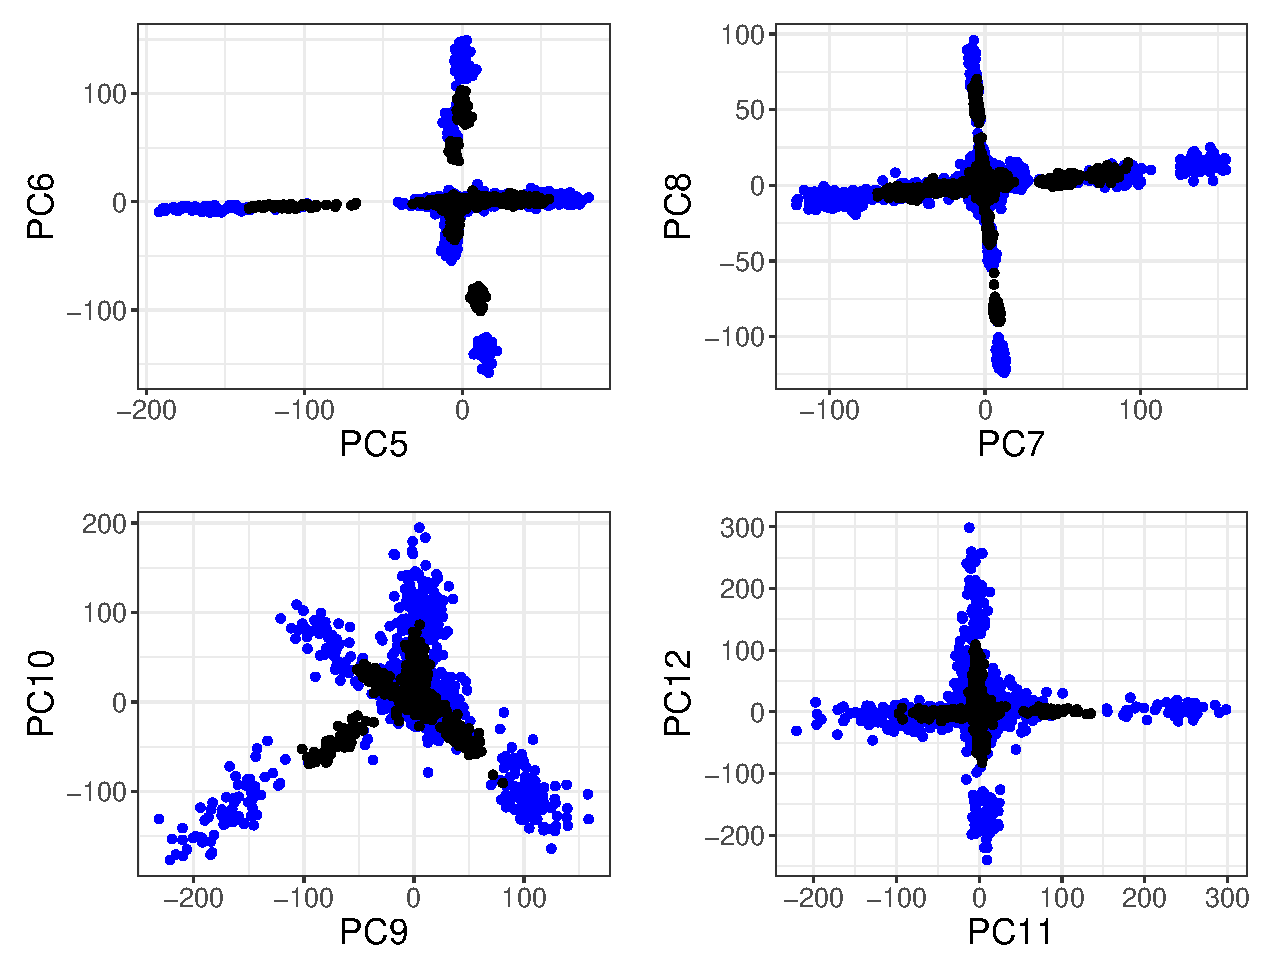
\includegraphics[width=0.9\textwidth]{proj1000G-related.pdf}}
\caption{Principal Component (PC) scores 5 to 12 of the 1000 Genomes project.
Black points are the 60\% individuals used for computing PCA.
Blue points are the same 60\% individuals, projected using the Online Augmentation, Decomposition, and Procrustes (OADP) transformation.
\label{fig:proj1000G-4}}
\end{figure}

\begin{figure}[!htpb]
\centerline{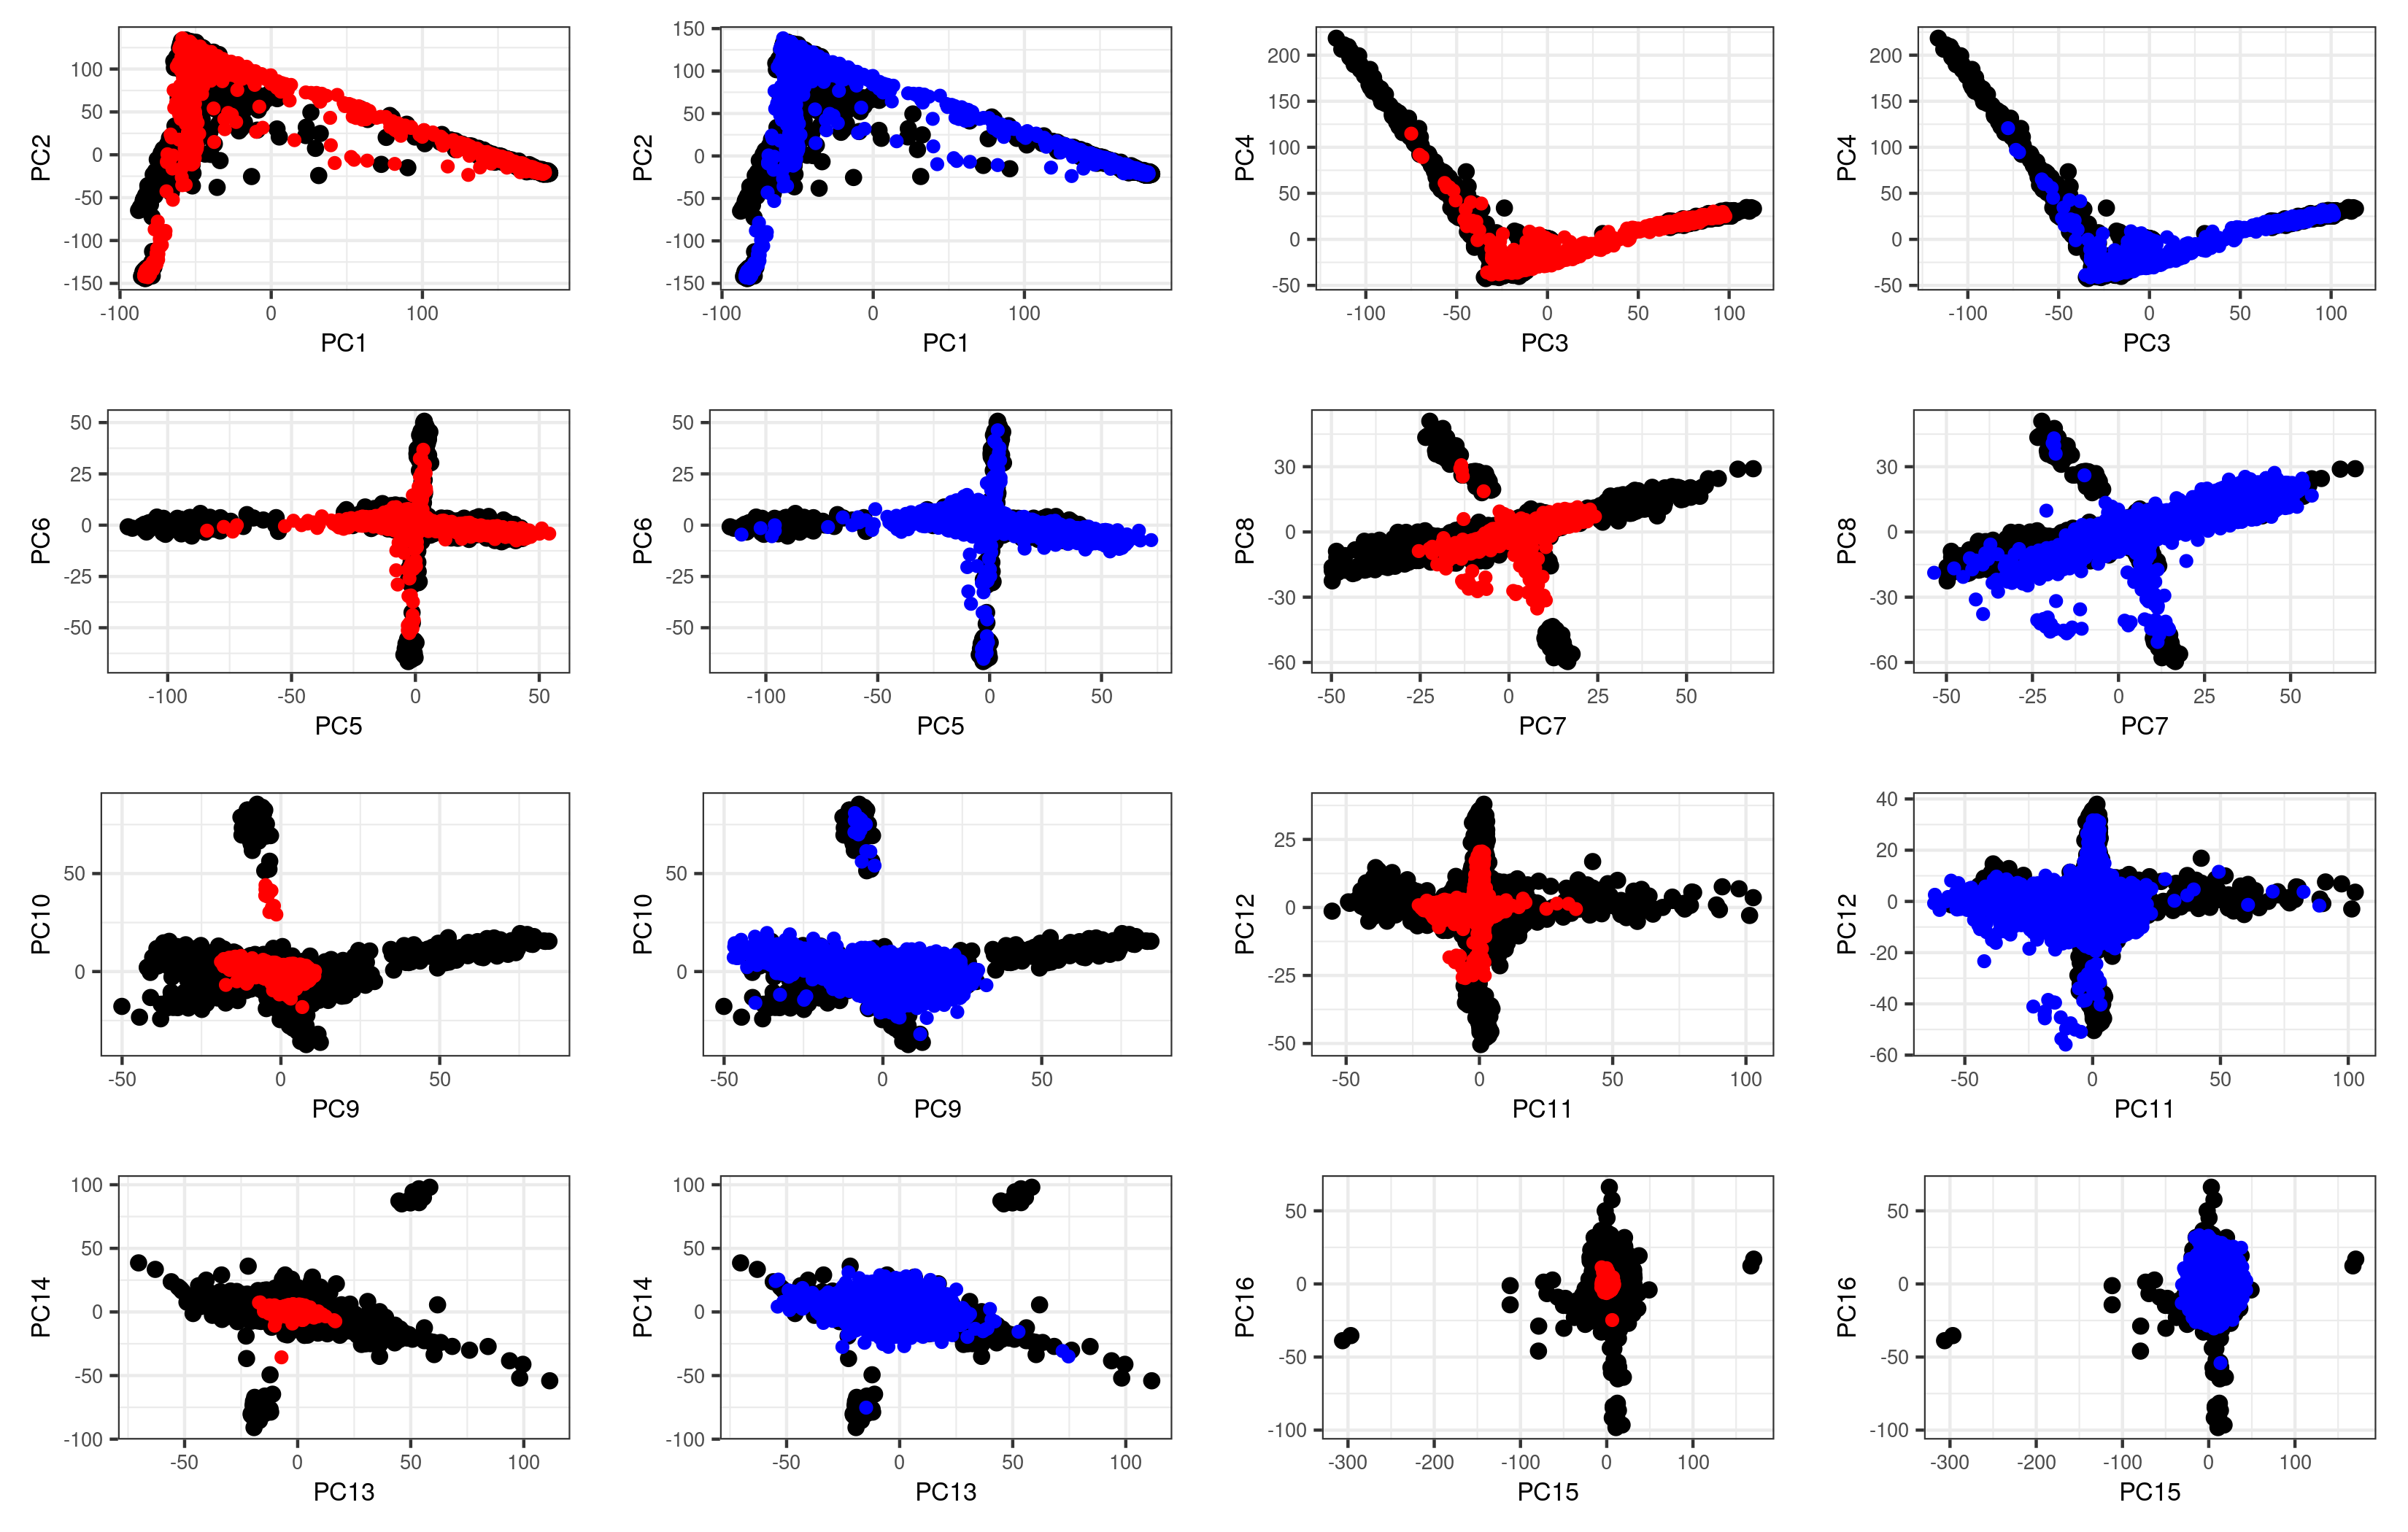
\includegraphics[width=0.9\textwidth]{proj1000G-UKBB.png}}
\caption{Principal Component (PC) scores 1 to 16 of the 1000 Genomes project and projected individuals from the UK Biobank.
Black points are PC scores of 1000G individuals used for computing PCA.
Blue points are the 488,371 individuals from the UK Biobank, projected using the Online Augmentation, Decomposition, and Procrustes (OADP) transformation. Note that only 20,000 random individuals are represented in this plot.
\label{fig:proj1000G-5}}
\end{figure}

\vspace*{1em}

\begin{figure}[!htpb]
\centerline{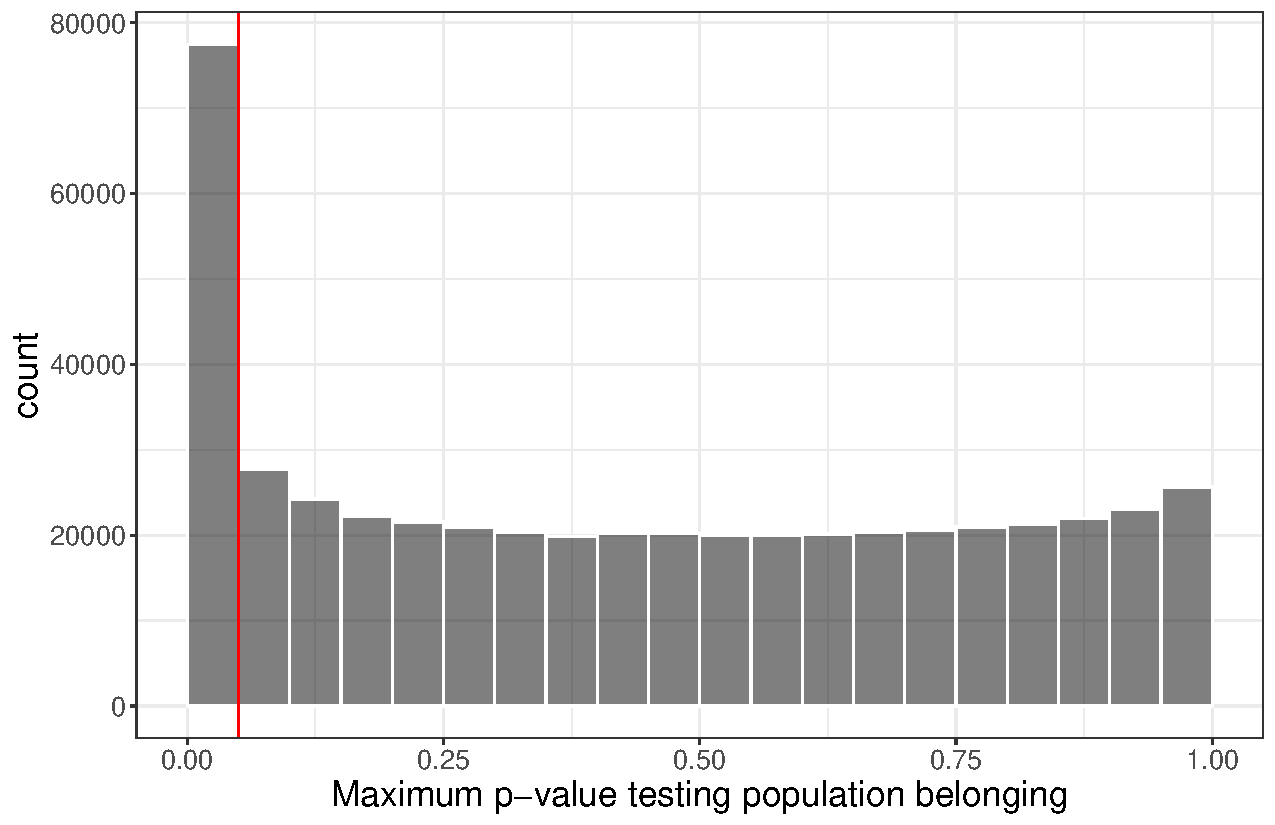
\includegraphics[width=0.8\textwidth]{hist-pval-max.pdf}}
\caption{Maximum p-values based on robust Mahalabonis distances of UK Biobank individuals from each of the 26 1000G populations.
\label{fig:ancestry-pval}}
\end{figure}

%%%%%%%%%%%%%%%%%%%%%%%%%%%%%%%%%%%%%%%%%%%%%%%%%%%%%%%%%%%%%%%%%%%%%%%%%%%%%%%%

% latex table generated in R 3.6.0 by xtable 1.8-4 package
% Sat Oct 19 00:18:24 2019
\begin{table}[ht]
\centering
\caption{Ancestry (left) of POPRES individuals and their matching to 1000G populations (top) by our method. See the description of 1000G populations at \url{https://www.internationalgenome.org/category/population/}.} 
\label{tab:ancestry-pred-popres}
\begin{tabular}{|l|c|c|c|c|c|}
  \hline
 & EUR\_CEU & EUR\_GBR & EUR\_IBS & EUR\_TSI & NA \\ 
  \hline
Anglo-Irish Isles & 159 & 57 &  &  & 50 \\ 
  Belgium & 28 & 3 &  &  & 12 \\ 
  Central Europe & 3 &  &  & 1 & 51 \\ 
  Eastern Europe & 2 &  &  &  & 28 \\ 
  France & 14 &  & 13 &  & 62 \\ 
  Germany & 37 &  &  &  & 34 \\ 
  Italy &  &  & 12 & 19 & 188 \\ 
  Netherlands & 10 & 2 &  &  & 5 \\ 
  Scandinavia & 5 &  &  &  & 10 \\ 
  SE Europe &  &  &  & 5 & 89 \\ 
  SW Europe &  &  & 193 &  & 71 \\ 
  Switzerland & 33 & 1 & 6 &  & 182 \\ 
   \hline
\end{tabular}
\end{table}

% latex table generated in R 3.6.0 by xtable 1.8-4 package
% Sat Oct 19 00:28:24 2019
\begin{table}[ht]
\centering
\caption{Ancestry (left) of Celiac individuals and their matching to 1000G populations (top) by our method. See the description of 1000G populations at \url{https://www.internationalgenome.org/category/population/}.} 
\label{tab:ancestry-pred-celiac}
\begin{tabular}{|l|c|c|c|c|c|c|c|}
  \hline
 & AMR\_MXL & EUR\_CEU & EUR\_FIN & EUR\_GBR & EUR\_IBS & EUR\_TSI & NA \\ 
  \hline
Finland &  & 4 & 1543 & 1 &  & 1 & 922 \\ 
  Italy &  &  &  &  & 15 & 229 & 795 \\ 
  Netherlands &  & 802 &  & 382 & 1 &  & 463 \\ 
  UK & 1 & 2865 & 1 & 2532 & 4 & 5 & 1346 \\ 
   \hline
\end{tabular}
\end{table}


\end{document}
